%  sample eprint article in LaTeX           --- M. Peskin, 9/7/00
%  modified for LHCP2017, lhcp2017@sjtu.edu.cn
%  This file is part of a tar file, which can be downloaded from the LHCP2017 indico site. 
%   https://indico.cern.ch/event/517784/overview 
% 


\documentclass[10pt]{article}
\usepackage{graphicx}



%%%%%%%%%%%%%%%%%%%%%%%%%%%%%%%%%%%%%%%%%%%%%%%%%%%%%%%%%%%%%%%%%%%%%%%%%%%%
%   document style macros
%%%%%%%%%%%%%%%%%%%%%%%%%%%%%%%%%%%%%%%%%%%%%%%%%%%%%%%%%%%%%%%%%%%%%%%%%%%%
\def\Title#1{\begin{center} {\Large #1 } \end{center}}
\def\Author#1{\begin{center}{ \sc #1} \end{center}}
\def\Address#1{\begin{center}{ \it #1} \end{center}}
\def\andauth{\begin{center}{and} \end{center}}
\def\submit#1{\begin{center}Submitted to {\sl #1} \end{center}}
\newcommand\pubblock{\rightline{\begin{tabular}{l} Proceedings of the Fifth Annual LHCP\\ 
         \pubdate  \end{tabular}}}

\newenvironment{Abstract}{\begin{quotation} \begin{center} 
             \large ABSTRACT \end{center}\bigskip 
      \begin{center}\begin{large}}{\end{large}\end{center} \end{quotation}}

\newenvironment{Presented}{\begin{quotation} \begin{center} 
             PRESENTED AT\end{center}\bigskip 
      \begin{center}\begin{large}}{\end{large}\end{center} \end{quotation}}

\def\Acknowledgements{\bigskip  \bigskip \begin{center} \begin{large}
             \bf ACKNOWLEDGEMENTS \end{large}\end{center}}
%%%%%%%%%%%%%%%%%%%%%%%%%%%%%%%%%%%%%%%%%%%%%%%%%%%%%%%%%%%%%%%%%%%%%%%%%%%%
%  personal abbreviations and macros
%    the following package contains macros used in this document:
\input econfmacros.tex
%%%%%%%%%%%%%%%%%%%%%%%%%%%%%%%%%%%%%%%%%%%%%%%%%%%%%%%%%%%%%%%%%%%%%%%%%%%

\textwidth=6.5in  \textheight=8.75in
\hoffset=-.85in
\voffset=-0.6in

%%  DO NOT CHANGE anything above.

% include packages you will need
\usepackage{color}

%%%%%%%%%%%%%%%%%%%%%%%%%%%%%%%%%%%%%%%%%%%%%%%%%%%%%%%%%%%%%%%%%%%%
% basic data for the eprint:
%%%%%%%%%%%%%%%%%%%%%%%%%%%%%%%%%%%%%%%%%%%%%%%%%%%%%%%%%%%%%%%%%%%%

% Instruction:
% Please change each of the following fields:
%

%% date
\newcommand\pubdate{\today}

%%  Affiliation
\def\affiliation{
On behalf of the CMS Collaboration, \\
Department of Physics \\
University of Wisconsin -- Madison, Madison, WI 53706-1390, USA}

\begin{document}

% large size for the first page
\large
\begin{titlepage}
\pubblock


%% Change the title, name, abstract
%% Title 
\vfill
\Title{  Multi-boson Measurements in CMS }
\vfill

%  if you need to add the support use this, fill the \support definition above. 
%   \Author{ FIRSTNAME LASTNAME \support }
\Author{ Kenneth Long }
\Address{\affiliation}
\vfill
\begin{Abstract}

Recent results from the CMS experiment on the simultaneous 
production of multiple vector bosons in proton-proton collisions at the 
CERN LHC are presented. Measurements of $WZ$ and $ZZ$ production with 
fully leptonic decays, $Z(\nu\nu)\gamma$, and 
WV ($V = W,Z \rightarrow q\bar{q}$) production at 8 and 13 TeV are discussed. 
Selected cross section measurements, unfolded differential measurements, and 
limits on anomalous triple gauge couplings
are presented and compared with theoretical predictions.


\end{Abstract}
\vfill

% DO NOT CHANGE 
\begin{Presented}
The Fifth Annual Conference\\
 on Large Hadron Collider Physics \\
Shanghai Jiao Tong University, Shanghai, China\\ 
May 15-20, 2017
\end{Presented}
\vfill
\end{titlepage}
\def\thefootnote{\fnsymbol{footnote}}
\setcounter{footnote}{0}
%

% normal size for the rest
\normalsize 

%% Your paper should be entered below. 

\section{Introduction}

Measurements of the production of multiple vector bosons in proton-proton collisions 
at the CERN LHC is an important test of the electroweak sector of
the Standard Model (SM). Such final states provide a natural probe of the 
vector boson self-couplings, which arise due to the non-Abelian nature of the
electroweak gauge group and are exactly predicted by the SM. Deviations from these
predictions could therefore be an indication of new physics. In addition,
due to recent theoretical developments, the production cross sections 
of all proton-proton processes producing vector boson pairs are
known at next-to-next-to-leading order in QCD, many differentially. 
When the perturbative QCD corrections are significant with respect to the experimental
uncertainties, measurements can directly validate the higher-order perturbative QCD
calculations.

This report summarizes recent measurements from the CMS collaboration, using
data collected by the CMS detector at $\sqrt{s} =$ 8 and 13 TeV. A brief summary
of measurements for a variety of vector boson pairs and decays is presented, 
each offering a unique probe of the SM and possible new physics. Full details of 
the analyses can be found in the references.

%%%%%%%%%%%%%%%%%%%%%%%%%%%%%%%%%%%%%%%%%%%%%%%%%%%%%%%%%%%%%%%%%%%%%%%%%
%%
%%   use this format to include a LaTeX table  into your paper
%%
%\begin{table}[t]
%\begin{center}
%\begin{tabular}{l|ccc}  
%Patient &  Initial level($\mu$g/cc) &  w. Magnet &  
%w. Magnet and Sound \\ \hline
% Guglielmo B.  &   0.12     &     0.10      &     0.001  \\
% Ferrando di N. &  0.15     &     0.11      &  $< 0.0005$ \\ \hline
%\end{tabular}
%\caption{ place the caption here }
%\label{tab:table1}
%\end{center}
%\end{table}
%%%%%%%%%%%%%%%%%%%%%%%%%%%%%%%%%%%%%%%%%%%%%%%%%%%%%%%%%%%%%%%%%%%%%%%%%%%

\section{Differential and Inclusive Cross Section Measurements}
\subsection{$Z(\nu\nu)\gamma$ Production}
\begin{figure}[htb]
  \centering
    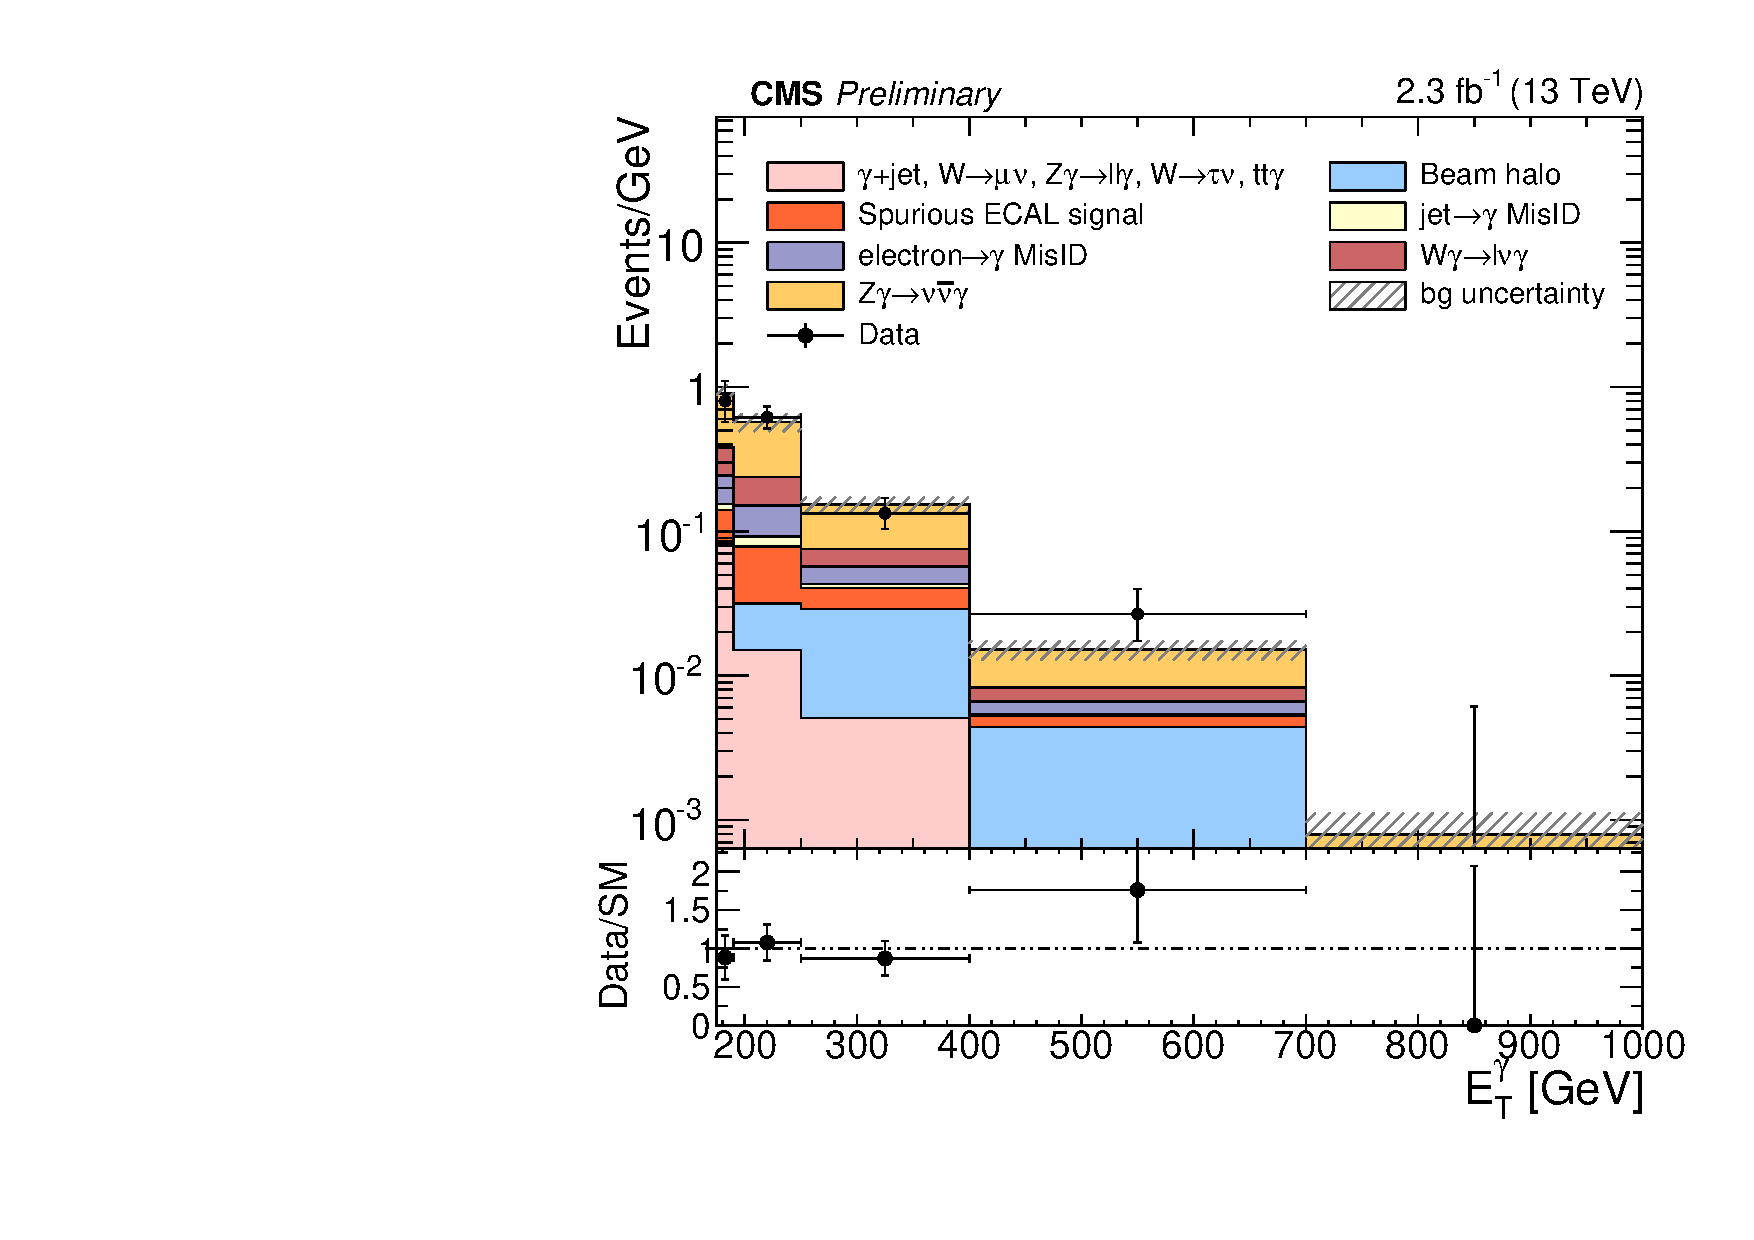
\includegraphics[height=2in]{figures/MonoPhoto_ETmiss.pdf}
  \caption{ }
  \label{fig:zgamma_etmiss}
\end{figure}
See Figure \ref{fig:zgamma_etmiss}
\cite{CMS-PAS-SMP-16-004}

The production of a Z boson produced in association with a photon,
with the Z decaying to pair of neutrinos, can only be produced through
initial-state radiation of a photon from the incoming quarks in the standard model.
Other production mechanisms could only arise through trilinear gauge boson 
self-interaction couplings (TGCs) which could arise due to new physics. 
Measurements of this channel for high photon transverse energy are therefore
sensitive to new physics, and are also important as background measurements to
dark matter searches in the mono-photon channel.

The $pp \rightarrow Z\gamma \rightarrow \nu\bar{\nu}\gamma$ fiducial cross section 
has been measured for transverse energy $E_{T}^{\gamma} > 175$ GeV and photon pseudorapidity
$abs{\eta^{\gamma}} < $ 1.44 using 2.3 fb$^{-1}$ of data collected by the CMS experiment in 2015.
The analysis selects a well-identified photon with transverse energy $E_{T}^{\gamma}$

The primary backgrounds to the signal process are experimental in nature, including 
spurious signals in the electromagnetic calorimeter (ECAL), beam halo, and cosmic rays. 
These contributions all give rise to signals mimicking photons in the detector, 
with missing transverse momentum arising due to the 
condition that the transverse momentum of the event sum to zero. The contribution of
these backgrounds is estimated
by via exploiting their characteristic shape and timing in the ECAL. Other backgrounds 
enter the selection due to misidentification

The measured fiducial cross section of
\begin{equation}
  \sigma_{\mathrm{fid}}(pp \rightarrow Z\gamma \rightarrow \nu\bar{\nu}\gamma) = 66.5 \pm 13.6 \, \mathrm{(stat)} \pm 14.3 \, 
        \mathrm{(syst)} \pm 2.2 \, \mathrm{(lumi)} \,\mathrm{fb}
\end{equation}
is found to be in agreement with the standard model prediction of $65.5 \pm 3.3$ fb, computed at
NNLO with MATRIX. \cite{bleh}

\subsection{$W^{\pm}Z$ Production at 8 and 13 TeV}

Measurements of WZ production with fully leptonic decays probe the charged
gauge interactions of the SM. The relatively clean three-lepton final state
is balanced by a modestly high cross section, allowing a high statistics measurement 
with controlled systematics. The analysis selects events with three leptons and 
missing transverse momentum $p_{T}^{miss} > 30$ GeV. The mass of the 3 leptons
is required to have $m_{3\ell} > $ 100 GeV reject events $Z\gamma$ events where a photon
radiated from the leptonic Z decay is misidentified as an electron. Events with
a b-tagged jet are rejected to reduce $t\bar{t}$ background.

Backgrounds for this measurement are categorized into processes producing at least
three prompt isolated leptons ($\ell = e, \mu$), including ZZ, triboson, and 
$t\bar{t}\gamma$, and those processes where nonprompt
leptons from hadrons decaying to leptons inside jets or jets misidentified as isolated
leptons pass the signal selection, predominantly $t\bar{t}$ and Drell-Yan. 
The Nonprompt background is evaluated with a data-driven approach using 
control regions of events passing the full analysis selection,
with the exception that one, two, or three leptons pass relaxed identification 
and isolation requirements but fail the more stringent requirements applied to signal events.
These events are extrapolated into the signal region using per-lepton 
``tight to loose'' transfer factors
calculated from a sample of dijet events. Prompt backgrounds are evaluated using 
simulated samples. The Z$\gamma$ process is also estimated with simulation.


The production cross section has been measured by the CMS experiment at 7, 8, 
\cite{Khachatryan:2016poo}
and 13 TeV
\cite{Khachatryan:2016tgp}.
These measurements and their agreement with the SM
predictions, computed at NNLO in QCD with MATRIX and NLO in QCD with MCFM \cite{bleh}
are summarized in figure~\ref{WZfigs}, which also presents ATLAS results for comparison. 
Good agreement with the SM predictions
is observed. Some tension is seen in the 13 TeV measurement with 2.3 fb$^{-1}$
and the NNLO prediction, but we note that this measurement is statistically
limited and await a measurement with an increased 13 TeV dataset.

Differential measurements of WZ production, unfolded using the 
iterative d'Agostini \cite{bleh} method, are presented using 19.6 fb$^{-1}$
collected by the CMS experiment in 2012 at 8 TeV. These measurements allow for careful
comparisons of theoretical predictions in distributions sensitive 
to higher-order corrections, such as the Z boson transverse momentum, which is
shown in figure~\ref{WZfigs}.

\begin{figure}[htb]
  \centering
    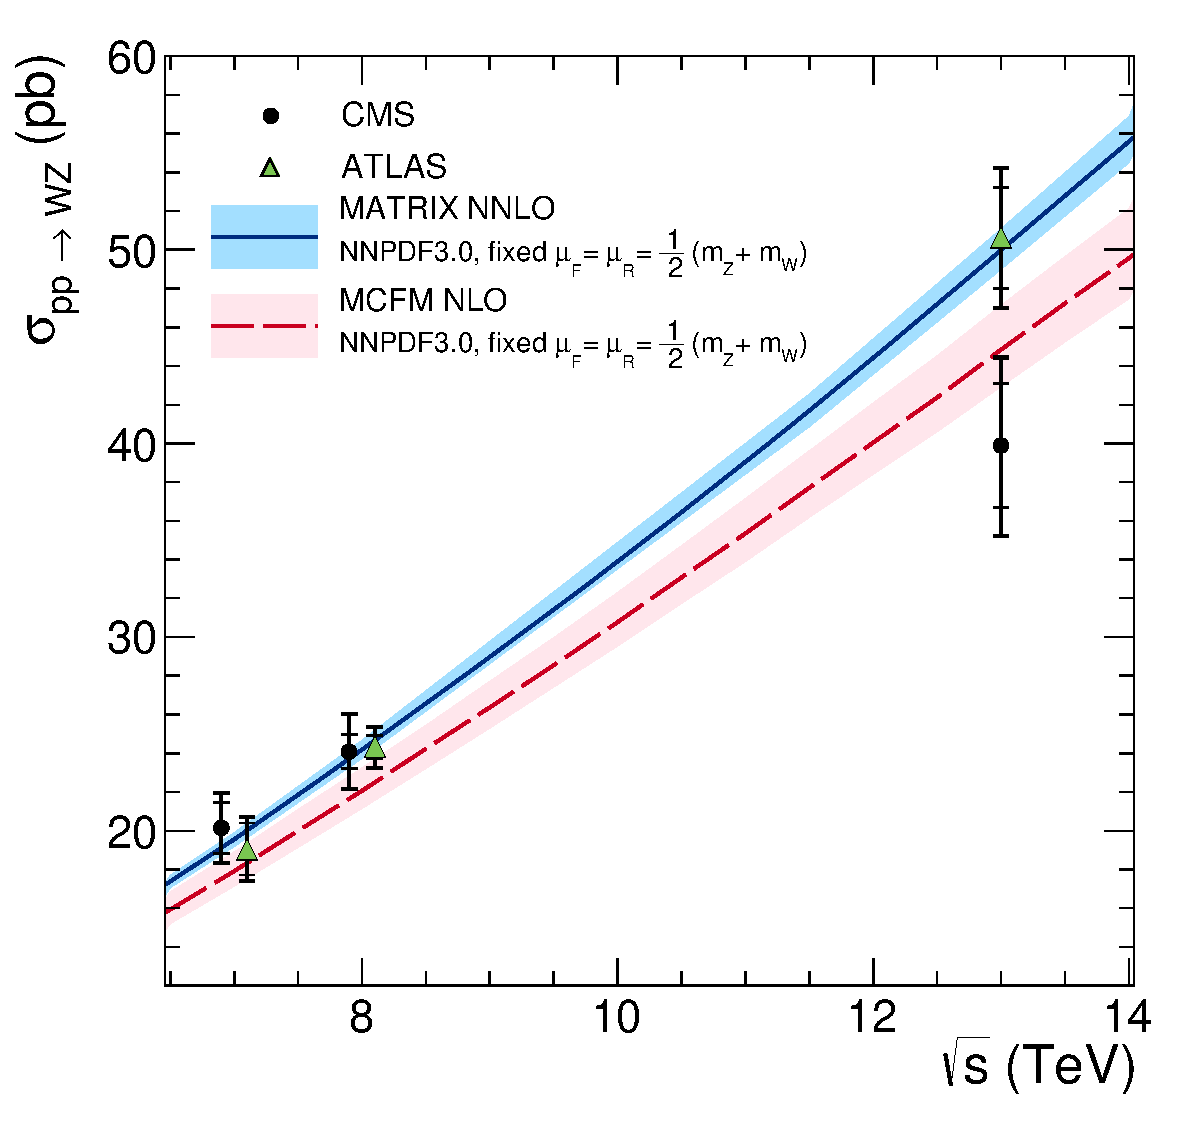
\includegraphics[height=2in]{figures/WZCrossSection_vs_sqrtS.pdf}
    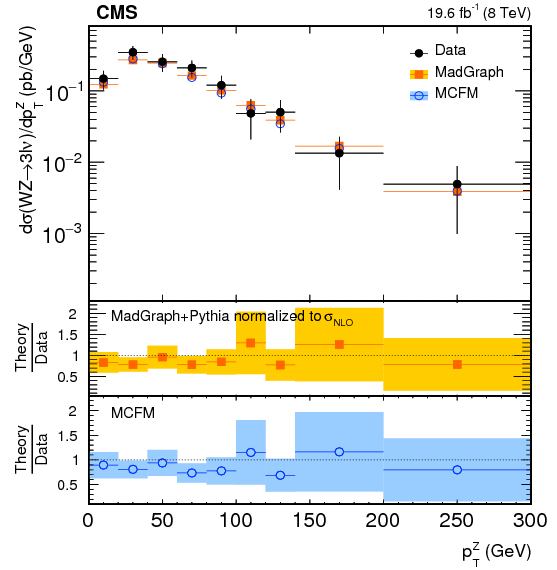
\includegraphics[height=2in]{figures/WZ8TeV_ptZ_unfolded.png}
    \caption{ (Left) The total $pp \rightarrow WZ$ cross section
      as of $\sqrt{s}$ measured by the CMS and 
      ATLAS experiments compared to the predictions of MCFM 7.0 and MATRIX v1.0.0\_beta4. 
      The CMS 13 TeV cross section are calculated for the Z boson mass window $60 - 120$ GeV. 
      The CMS 7 and 8  TeV  cross sections are calculated for the Z boson mass window $71 - 111$ GeV.
      ATLAS measurements are performed with the Z boson mass window $66 - 116$  GeV.
      (Right) Differential cross section at $sqrt{s} = 8$ TeV as a function
      of the Z boson transverse momentum,
      compared to
      the fixed-order prediction from MCFM 6.3 and the prediction from
      MadGraph5.1+Pythia6.4, using MLM merging of tree-level contributions 
      for up to two additional partons.
      }
  \label{fig:WZfigs}
\end{figure}

\subsection{$ZZ$ Production}

In spite of its low cross section, the $ZZ \rightarrow 4\ell$ process 
is favorable experimentally due to its clean and fully reconstructed 
four-lepton final state. It provides a probe of the neutral gauge sector 
of the standard model, and its role as the primary background to the SM Higgs
boson in the four lepton channel makes it an important SM 
process to understand.

\begin{figure}[htb]
  \centering
    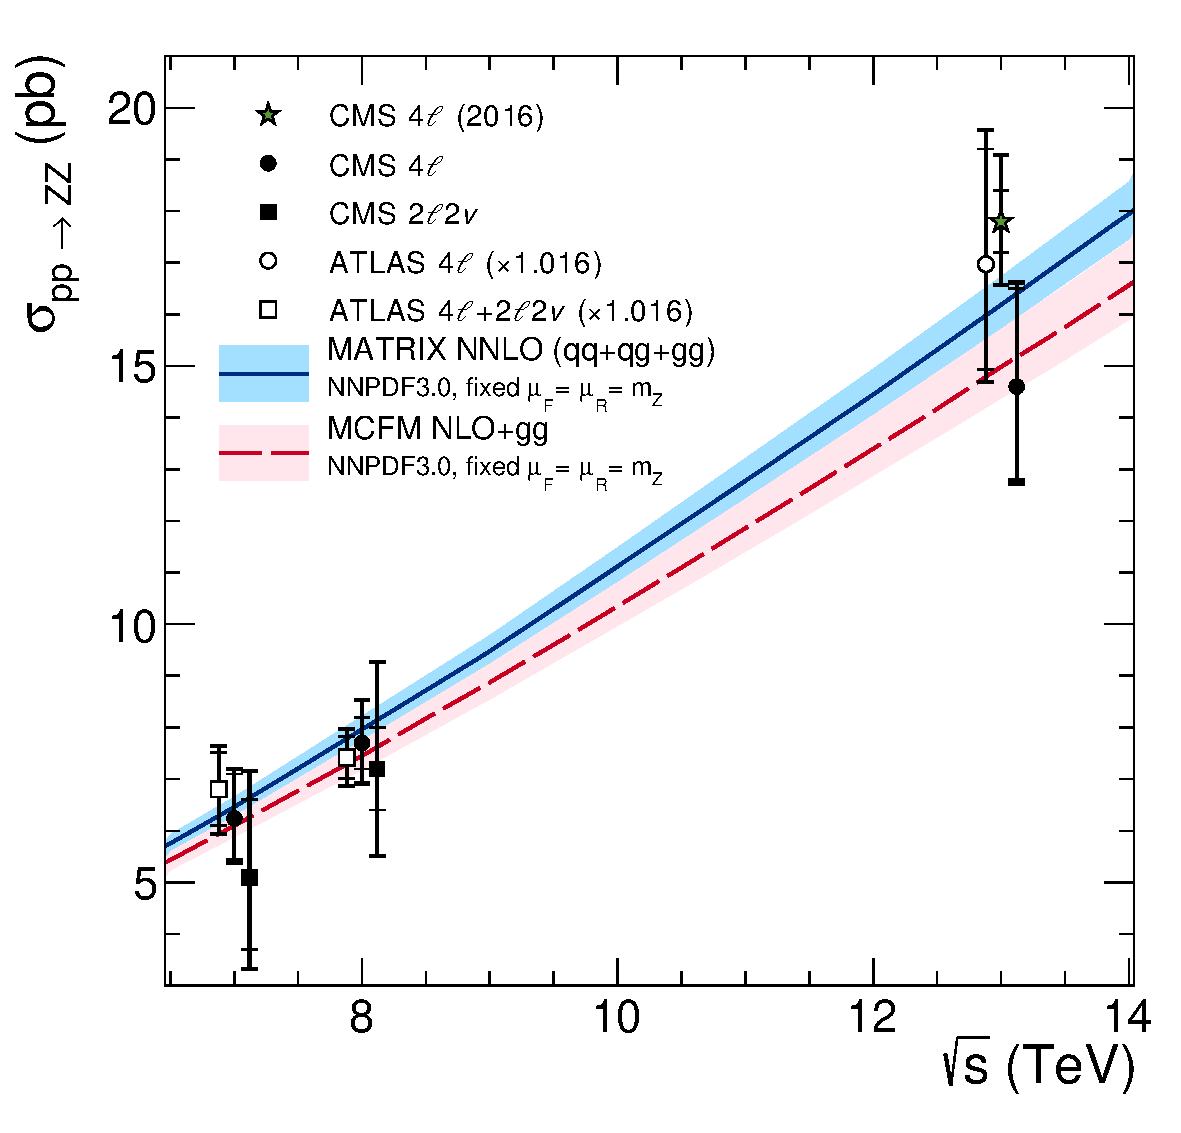
\includegraphics[height=2in]{figures/ZZCrossSection_vs_sqrtS.pdf}
    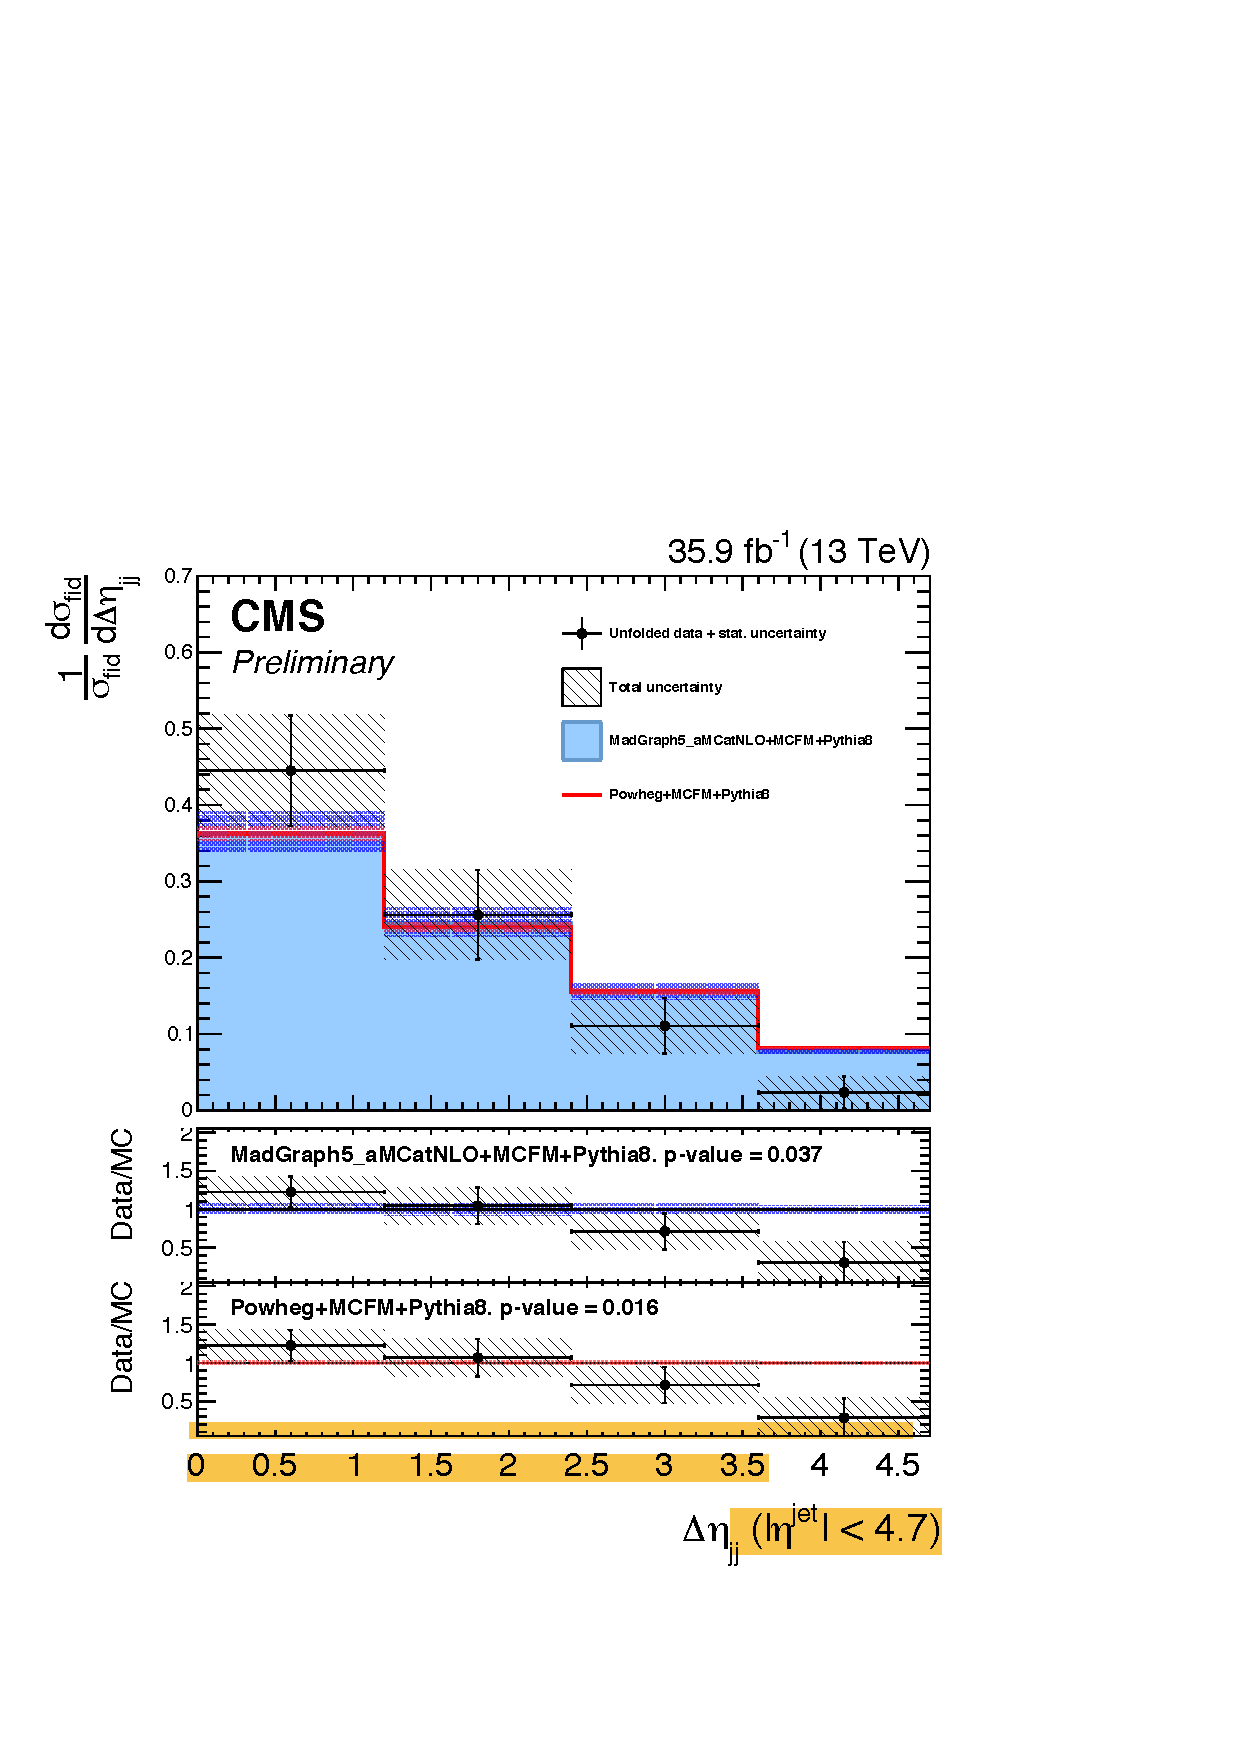
\includegraphics[height=2in]{figures/ZZ_13TeV_dEtajj_unfolded.pdf}
  \caption{ Place the caption here}
  \label{fig:ZZinclusive}
\end{figure}

The analysis selects 4 leptons forming two composite Z boson candidates with
mass in the range $60 < m_{\ell^{+}\ell^{-}} 120$ GeV. The very low background
in this channel allows only loose identification and isolation criteria to 
be required. Backgrounds with four prompt leptons such as triboson and $t\bar{t}V$, 
which have very
low production cross sections, are evaluated using simulated samples. The 
contribution from nonprompt leptons are estimated using the same technique
described for WZ in the previous section, however, the ``tight to loose'' transfer 
factors are derived using a sample of Drell-Yan events, using associated 
jets as the loose and tight lepton probe.

Briefly describe results yo


\begin{figure}[htb]
  \centering
    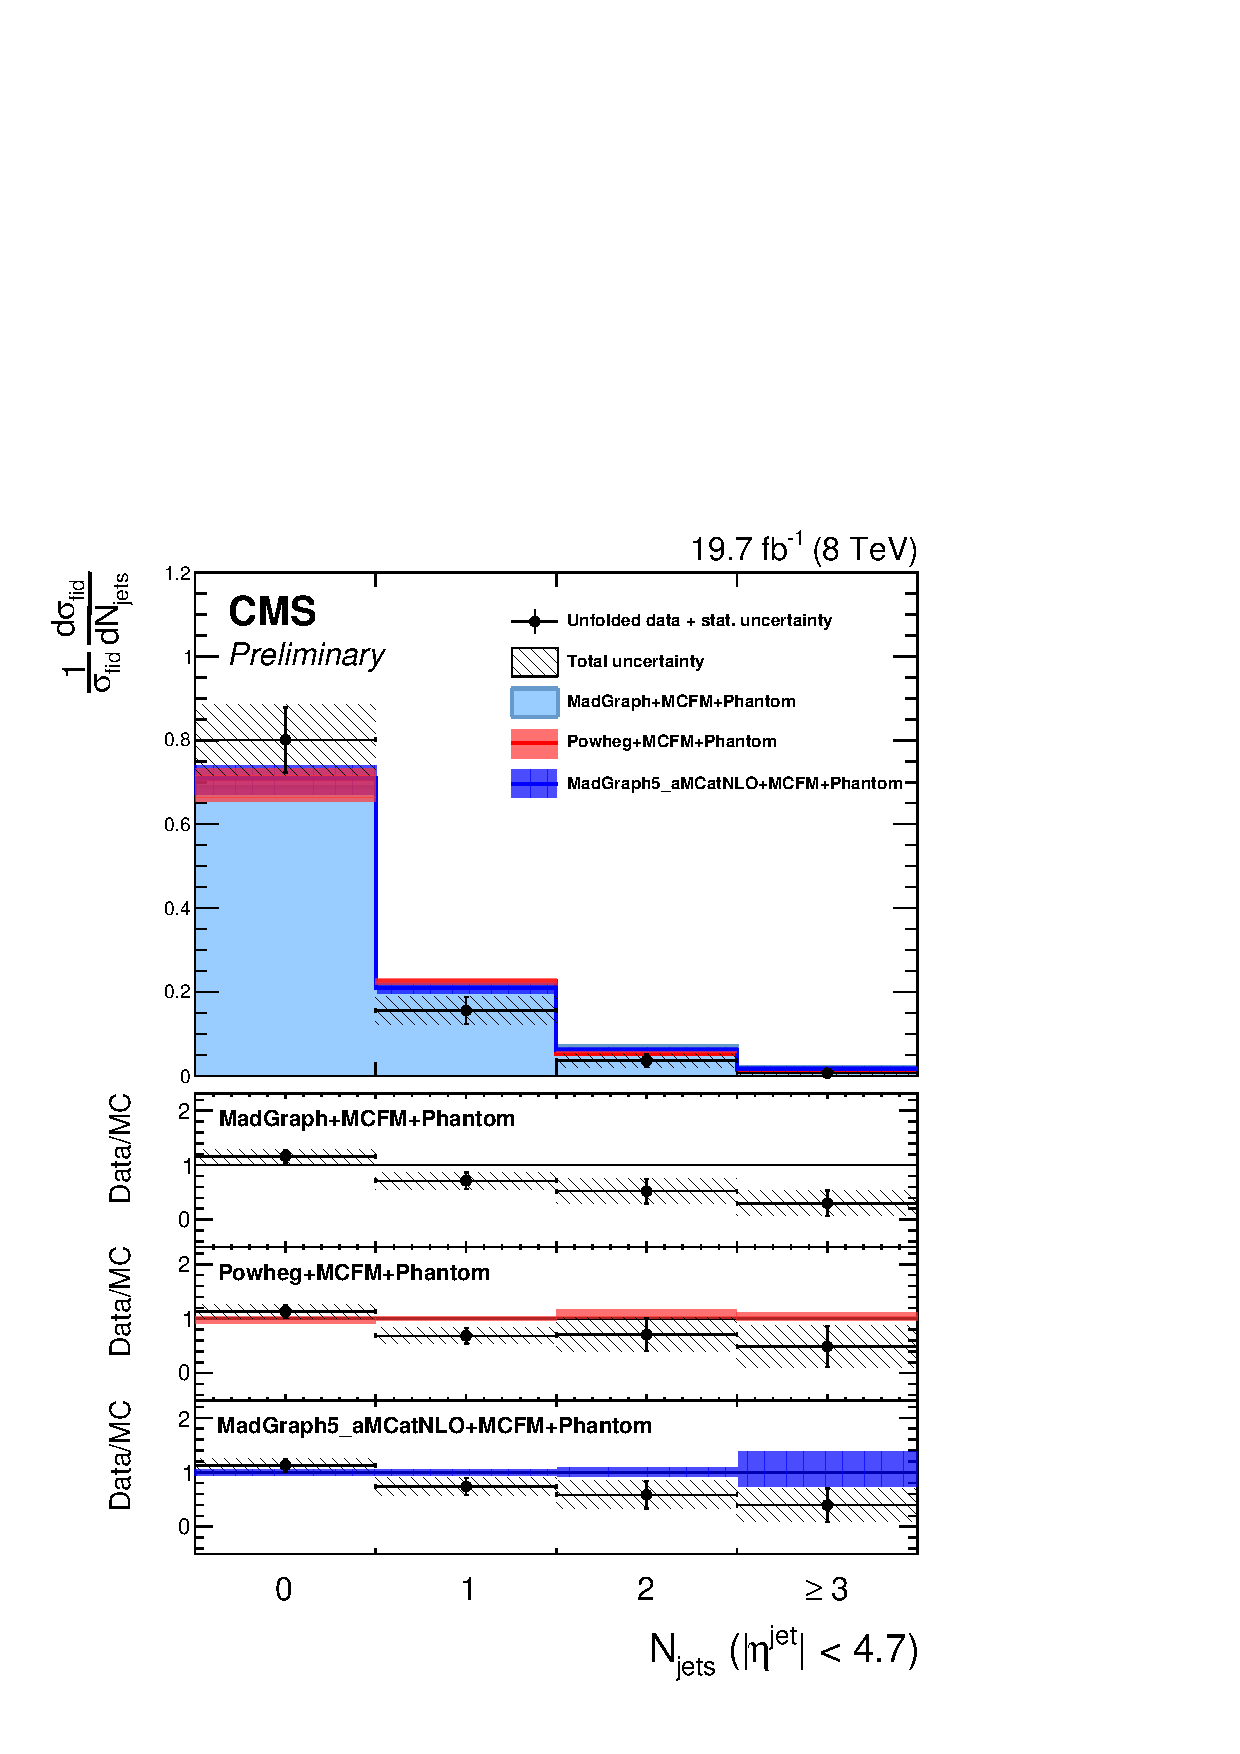
\includegraphics[height=2in]{figures/ZZ_8TeV_nJets_unfolded.pdf}
    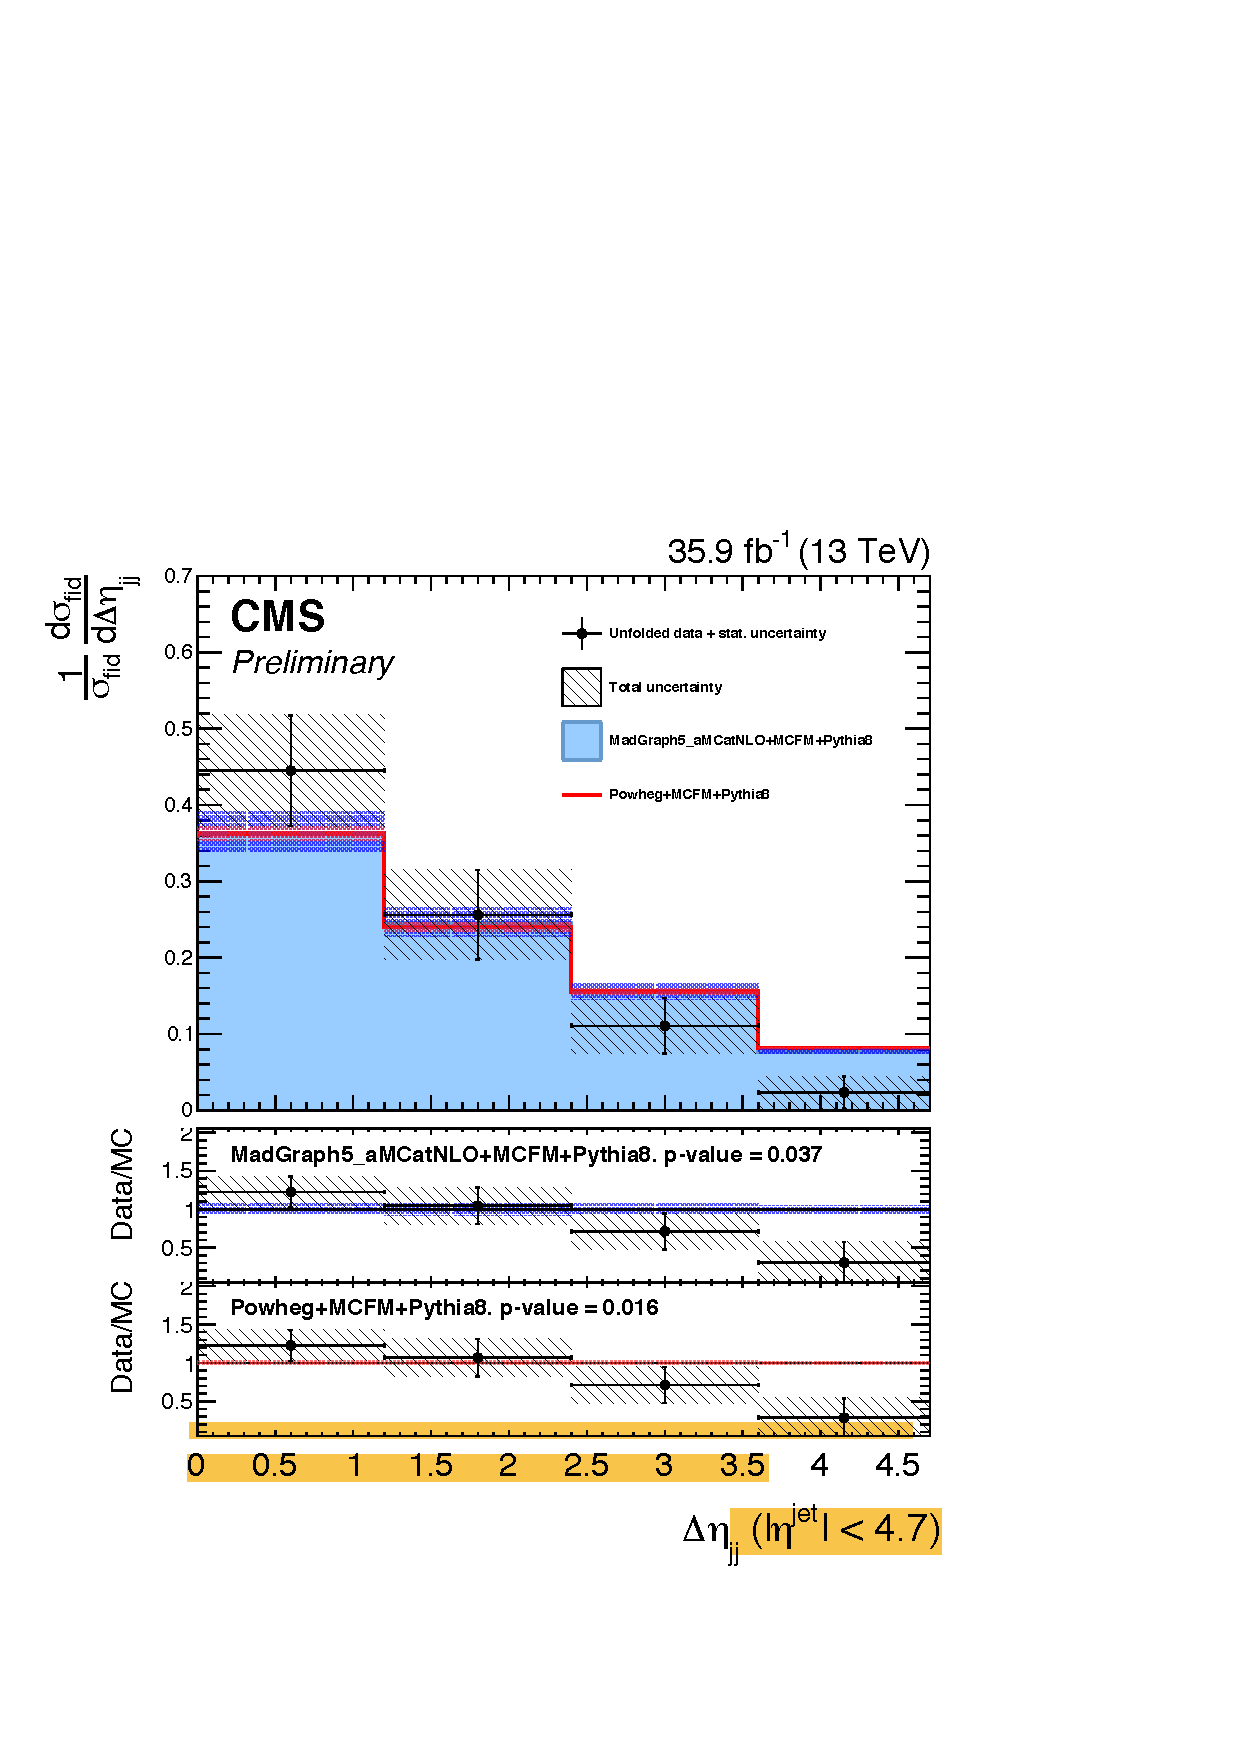
\includegraphics[height=2in]{figures/ZZ_13TeV_dEtajj_unfolded.pdf}
  \caption{ Place the caption here}
  \label{fig:ZZjets}
\end{figure}
\cite{CMS:2017ruh}
\cite{CMS-PAS-SMP-16-019}

Describe jets, motivation, and results yo

\section{Limits on Anomalous Gauge Couplings}

\subsection{Limits from $WV$ Production with Semi-leptonic Decays}

Describe anlaysis and limits

\cite{CMS:2017ruh}
\cite{Sirunyan:2017bey}

\begin{figure}[htb]
  \centering
    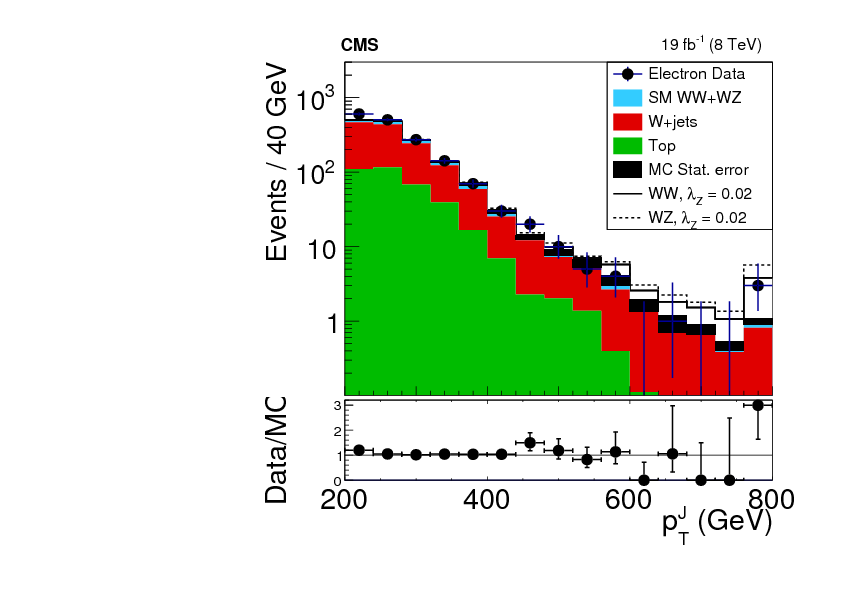
\includegraphics[height=2in]{figures/WV8TeV_ptJ_aC.png}
    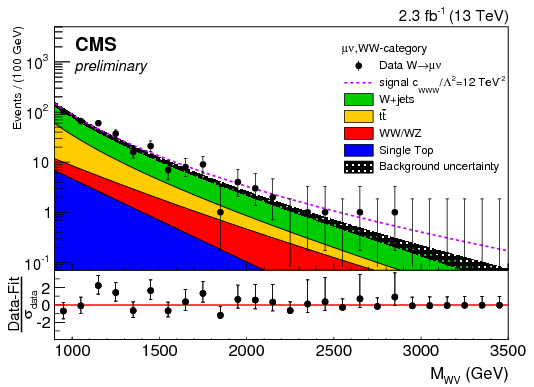
\includegraphics[height=2in]{figures/WV13TeV_mWW_aC.png}
  \caption{ Place the caption here}
  \label{fig:zgamma_etmiss}
\end{figure}

\subsection{Limits from Diboson States with Fully Leptonic Decays}

Briefly dump some plots I guess

\section{Conclusions}

Very brief, maybe a summary plot
...... \cite{CMS:2016djf} \cite{Cascioli:2014yka} 

\bibliographystyle{JHEP}
\bibliography{bibliography}
\end{document}
